\section{矩阵分解}

\subsection{矩阵的三角分解}
\subsubsection{基本知识}
 \begin{enumerate}
\item (单位)正线上(下)三角复(实)矩阵
\item 上三角矩阵$R$ 的逆$R^{-1}$也是上三角矩阵,且对角元是$R$对角元的倒数
\item 两个上三角矩阵$R_1,R_2$的乘积也是上三角矩阵,且对角元是$R_1$与$R_2$对角元之积;
\item	酉矩阵$U$ 的逆$U^{-1}$也是酉矩阵
\item 两个酉矩阵之积$U_1U_2$也是酉矩阵
\end{enumerate}


\subsubsection{n阶矩阵的QR分解和上下三角分解}

\begin{theorem}
\begin{enumerate}
\item\colorbox{yellow}{$A\in C^{n\times n}_n \Rightarrow A=U_1R=LU_2$(\textcolor{red}{唯一表示}),   其中$L(R)$是正线下(上)复矩阵,}
\colorbox{yellow}{$U_1,U_2$为酉矩阵$(U_1^HU_1=E,U_1\in C^{n\times n}_n)$.}
\item \colorbox{yellow}{$A\in R^{n\times n}_n \Rightarrow A=Q_1R=LQ_2$(\textcolor{red}{唯一表示}), 其中$L(R)$是正线下(上)三角复矩阵,  }

\colorbox{yellow}{$Q_1,Q_2$为正交矩阵.}

\item \colorbox{yellow}{$A\in C^{n\times n}_n,A^H=A$且正定$\Rightarrow A=P^HP(\mbox{表示法不唯一,且}P\mbox{可逆})$}

\hspace{5.85cm}\colorbox{yellow}{$= R^HR(\mbox{表示法唯一,且}R\mbox{是正线上三角复矩阵})$}

\item \colorbox{yellow}{$A\in R^{n\times n}_n,A$实对称且正定$\Rightarrow A=P^HP(\mbox{表示法不唯一,且}P\mbox{可逆})$}

\hspace{5.9cm}\colorbox{yellow}{$= R^HR(\mbox{表示法唯一,且}R\mbox{是正线上三角实矩阵})$}
\end{enumerate}
\end{theorem}
\begin{note}
3阶方阵QR分解:
	
	$A=(\alpha_1,\alpha_{2},\alpha_3)$可逆,则施密特正交化得
	\begin{align*}
		&\beta_1=\alpha_1  & \xi_1=\dfrac{\beta_1}{\|\beta_1\|}\\
		&\beta_2=\alpha_{2}-\dfrac{(\alpha_2,\beta_1)}{(\beta_1,
			\beta_1)}\beta_1& \xi_2=\dfrac{\beta_2}{\|\beta_2\|}\\
		&\beta_3=\alpha_{3}-\dfrac{(\alpha_3,\beta_1)}{(\beta_1,
			\beta_1)}\beta_1-\dfrac{(\alpha_3,\beta_2)}{(\beta_2,
			\beta_2)}\beta_2& \xi_2=\dfrac{\beta_3}{\|\beta_3\|}
	\end{align*}
$Q=\begin{pmatrix}
	\xi_1&\xi_2&\xi_3
\end{pmatrix}\quad
R=\begin{pmatrix}
	k_{11}& k_{21}&k_{23}\\
	0&k_{22}&k_{32}\\
	0&0&k_{33}
\end{pmatrix}\quad k_{ij}=\left\{\begin{array}{ll}
\|\beta_i\|&j=i\\
(\alpha_i,\xi_j)&j\ne i
\end{array}\right.
$



\end{note}

\begin{theorem}
设$A\in C^{n\times n}_n, L(\tilde{L})$为(\textcolor{red}{单位})下三角复矩阵,$R(\tilde{R})$为(\textcolor{red}{单位})上三角复矩阵,$D$为对角矩阵,则下列命题等价:
\begin{enumerate}
\item $A$的顺序主子式均不为0
\item $A=L\tilde{R}$(\textcolor{red}{唯一分解}),$l_{ii}\ne0(\forall i)$
\item $A=\tilde{L}R$(\textcolor{red}{唯一分解}),$r_{ii}\ne0(\forall i)$
\item $A=\tilde{L}D\tilde{R}$(\textcolor{red}{唯一分解}),$d_{ii}\ne0(\forall i)$
\end{enumerate}
\end{theorem}

\subsubsection{任意矩阵的QR分解}

\begin{enumerate}
\item\colorbox{yellow}{$A\in C^{m\times n}_m$($m<n,\mbox{行满秩}$)$\Rightarrow A=\begin{pmatrix}
	L&O\end{pmatrix}V=\begin{pmatrix}L&O\end{pmatrix}\begin{pmatrix}V_1\\V_2\end{pmatrix}$}

\colorbox{yellow}{其中,$L$是正线下三角复矩阵,$V\in C^{n\times n},V_1\in C^{m\times n}_m$}
 \begin{enumerate}
 \item	 $A$可以唯一分解为
 	\[
 		A=LU
 	\]
 	其中,$L$是$m$阶正线下三角矩阵,$U\in C^{m\times n}_m$
\end{enumerate}
\item\colorbox{yellow}{$A\in C^{m\times n}_n$($n<m,\mbox{列满秩}$)$\Rightarrow A=U\begin{pmatrix}
		R\\O\end{pmatrix}=\begin{pmatrix}U_1&U_2\end{pmatrix}\begin{pmatrix}
		R\\O\end{pmatrix}$}
	
	\colorbox{yellow}{其中,$R$是正线上三角复矩阵,$U\in C^{m\times m},U_1\in C^{m\times n}_n$}
	 \begin{enumerate}
		\item	 $A$可以唯一分解为
		\[
		A=UR
		\]
		其中,$R$是$n$阶正线上三角矩阵,$U\in C^{m\times n}_n$
	\end{enumerate}
\item \colorbox{yellow}{$A\in C^{m\times n}_r$},则存在酉矩阵$U\in U^{m\times m},V\in U^{n\times n}$及$r$阶正线下三角矩阵$L$,使得
\[\colorbox{yellow}{$
A=U\begin{bmatrix}
		L&0\\
		0&0
\end{bmatrix}V$}
\]

\end{enumerate}

\subsection{投影}
\subsubsection{投影的概念}
$L\oplus M=V_n(C)$直和$\Leftrightarrow \forall \alpha \in V_n(C),\alpha=\beta+\gamma,\beta \in L,\gamma \in M$唯一.
\[
P_{LM}\alpha=\beta,P_{LM}\beta =\beta \Rightarrow P_{LM}\alpha=\beta=P_{LM}\beta=P_{LM}P_{LM}\alpha\Rightarrow P_{LM}=P_{LM}^2
\]

\begin{figure}[H]
	\small
	\centering 
	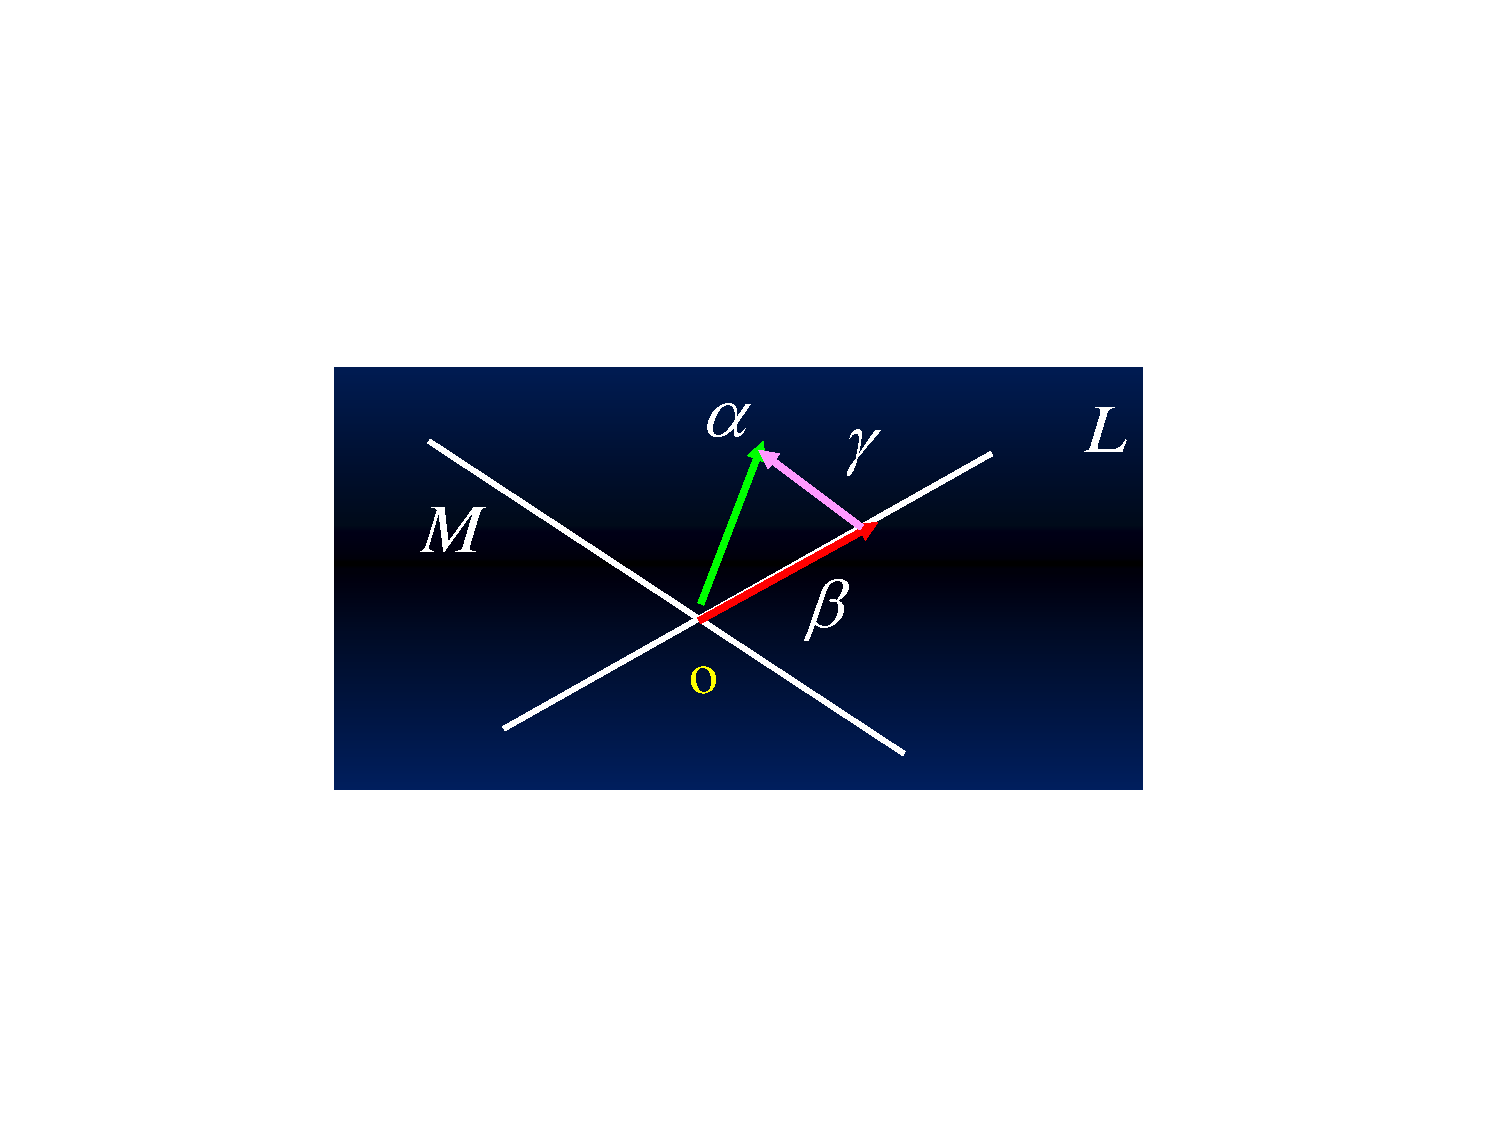
\includegraphics[scale=0.7]{image/CH3P2.pdf}  
	%\caption{信息包结构} 
	\label{fig1}  
\end{figure}



\[
\forall \begin{array}{c}
	\alpha_{1} \\
	\alpha_{2}
\end{array} \in V, \alpha \in V, k \in C \Rightarrow\left\{\begin{array}{c}
	P_{L M}\left(\alpha_{1}+\alpha_{2}\right)=P_{L M} \alpha_{1}+P_{L M} \alpha_{2} \\
	P_{L M}(k \alpha)=k \bullet P_{L M} \alpha
\end{array}\right.
\]

\subsubsection{投影变换与矩阵}
\[
\begin{array}{l}
	\left(\varepsilon_{1}, \varepsilon_{2}, \cdots, \varepsilon_{n}\right) A=P_{L M}\left(\varepsilon_{1}, \varepsilon_{2}, \cdots, \varepsilon_{n}\right)=P_{L M}^{2}\left(\varepsilon_{1}, \varepsilon_{2}, \cdots, \varepsilon_{n}\right) \\
	=P_{L M}\left(P_{L M}\left(\varepsilon_{1}, \varepsilon_{2}, \cdots, \varepsilon_{n}\right)\right)=P_{L M}\left(\left(\varepsilon_{1}, \varepsilon_{2}, \cdots, \varepsilon_{n}\right) A\right) \\
	=\left(P_{L M}\left(\varepsilon_{1}, \varepsilon_{2}, \cdots, \varepsilon_{n}\right)\right) A=\left(\varepsilon_{1}, \varepsilon_{2}, \cdots, \varepsilon_{n}\right) A \bullet A=\left(\varepsilon_{1}, \varepsilon_{2}, \cdots, \varepsilon_{n}\right) A^{2} \\
\colorbox{yellow}{$\Rightarrow A=A^{2}$(\mbox{幂等矩阵})}
\end{array}
\]

\subsubsection{正交投影与矩阵}
$V_n(C),\alpha=\beta+\gamma,\beta \in L,\gamma \in M$且$\beta\bot\gamma(\Leftrightarrow(\beta,\gamma)=0)$,则$\beta$为$\alpha$的正交投影.

正交投影矩阵满足:\colorbox{yellow}{$\Rightarrow A=A^{2}$(幂等矩阵)且$A=A^H$}

\subsubsection{幂等矩阵的性质}
$A\in C^{m\times n}$,则
\[
\begin{split}
	&\colorbox{yellow}{$\mbox{A的值域:} R(A)=\{y|y=Ax,\forall x\in C^{n}\}$}\\
	&\colorbox{yellow}{$\mbox{A的核:} N(A)=\{x|Ax=0,\forall x\in C^{n}\}$}
\end{split}
\]
\[
A\in C^{m\times n}\Rightarrow\left\{\begin{array}{l}
\colorbox{yellow}{$ \mathrm{dim}R(A)+\mathrm{dim}N(A^H)=m $}\\
\colorbox{yellow}{$ \mathrm{dim}R(A^H)+\mathrm{dim}N(A)=n $}\\
\colorbox{yellow}{$ C^m=R(A) \oplus N(A^H)$}\\
\colorbox{yellow}{$ C^n=R(A^H) \oplus N(A)$}\\
\end{array}\right.
\]
基本结论:
\[
A\in C^{n\times n}, A=A^2\Rightarrow\left\{\begin{array}{l}
	\colorbox{yellow}{$ A^H,(E-A)\mbox{幂等矩阵} $}\\
	\colorbox{yellow}{$ A\mbox{的特征值非0即1,且可对角化}$}\\
	\colorbox{yellow}{$ \mathrm{rank}(A)=\mathrm{tr}(A)$}\\
	\colorbox{yellow}{$ A(E-A)=(E-A)A=0$}\\
	\colorbox{yellow}{$ A\alpha=\alpha\Leftrightarrow \alpha \in R(A)$}\\
	\colorbox{yellow}{$ N(A)= R(E-A), R(A)=N(E-A)$}\\
\end{array}\right.
\]


\subsection{矩阵的谱分解}


\subsubsection{单纯矩阵的谱分解}
\begin{definition}
	若矩阵$A$的每个特征值的\colorbox{yellow}{代数重数等于几何重数},则矩阵$A$是\colorbox{yellow}{单纯矩阵}.
\end{definition}

\begin{theorem}
$A\in C^{n\times n}$是单纯矩阵$\Rightarrow A=\sum\limits_{i=1}^{n}\lambda_iA_i$(\textcolor{red}{$\Leftrightarrow A=\sum\limits_{i=1}^{k}\lambda_iA_i$})
其中:
\[
\colorbox{yellow}{$
\left\{\begin{array}{l}
	\lambda_i (i=1,2,\cdots,n)\mbox{是$A$的特征值}\\
	\left(\textcolor{red}{\lambda_i (i=1,2,\cdots,k)\mbox{是$A$的$k$个不同特征值}}\right)\\
	A_i\mbox{满足}
		\left\{\begin{array}{l}
			\mbox{幂等性:} A_i^2=A_i(A_i=x_iy_i^T,x_i\mbox{是$A_i$的特征向量},y_i\mbox{是$A_i^T$的特征向量})\\
			\mbox{分离性:} A_iA_j=0(j\ne i)\\
			\mbox{可加性:}\sum\limits_{i=1}^{n}A_i=E_n(\textcolor{red}{\sum\limits_{i=1}^{k}A_i=E_n})\\
		\end{array}\right.
\end{array}\right.
$}
\]
\end{theorem}


\begin{proof}
	由于$A$为单纯矩阵,则$A$有$n$个线性无光的特征向量
	
	设$Ax_i=\lambda_i x_i(i=1,2,\cdots, n)$,其中$x_i$为特征值$\lambda_i$对应的特征向量.令$P=(x_1,x_2,\cdots,x_n),P^{-1}=\begin{pmatrix}
		y_1^T\\y_2^T\\ \vdots \\ y_n^T
	\end{pmatrix}$,则$y_1^T,y_2^T, \cdots,  y_n^T$也线性无关.

\[A=P\mathrm{diag}(\lambda_{1},\lambda_{2},\cdots,\lambda_n)P^{-1}=\sum\limits_{i=0}^n\lambda_ix_iy_i^T=\sum\limits_{i=0}^n\lambda_iA_i,A_i=x_iy_i^T\]
\[
P^{-1}P=E\Rightarrow y_i^Tx_i=\left\{\begin{array}{ll}
1&j=i\\
0&j\ne i
\end{array}\right.\Rightarrow A_iA_i=x_iy_i^Tx_iy_i^T=A_i\Rightarrow \mbox{$A_i$为幂等矩阵}
\]
\begin{note}
	$A^n=\sum\limits_{i=0}^n\lambda_i^nx_iy_i^T=\sum\limits_{i=0}^n\lambda_i^nA_i$
\end{note}
\end{proof}



\subsubsection{正规矩阵的谱分解}
\begin{definition}
$A\in C^{n\times n}$满足
\colorbox{yellow}{$ AA^H=A^HA  $}
则称$A$为\colorbox{yellow}{正规矩阵}(正规矩阵不一定是Hermite矩阵).
\end{definition}
\noindent 几种正规矩阵:
\begin{enumerate}
\item $A^H=A \Rightarrow$$A$正规
\item $A^H=-A \Rightarrow$$A$正规
\item $A^H=\mathrm{diag}(a_1,a_2,\cdots,a_n) \Rightarrow$$A$正规
\item $U\in C^{n\times n},U^HU=UU^H=E\Rightarrow U$正规
\end{enumerate}
\noindent $A$为正规矩阵,则:


\begin{enumerate}
	\item 存在$U$矩阵,使得$U^HAU$和$U^HA^HU$均为对角矩阵(定理\ref{jjj})
	\item $A$为单纯矩阵
	\item 若$Ax=\lambda_ix(x\ne 0),$则$A^Hx=\bar{\lambda_i}x$
	\item $A$不同特征值对应的特征向量必然正交.
	\begin{proof}
		设不相同特征值$\lambda,\mu$对应得特征向量分别为$x,y$,则$Ax=\lambda x,Ay=\mu y$
		\[\begin{split}
			&\bar{\lambda}(x,y)=(\lambda x,y)=(Ax,y)=(x,A^{H}y)=(x,\bar{\mu}y)=\bar{\mu}(x,y)\\
			&\Rightarrow (\bar{\lambda}-\bar{\mu})(x,y)=0,(\bar{\lambda}-\bar{\mu})\ne0 \Rightarrow(x,y)=0
		\end{split}
		\]
	\end{proof}
\end{enumerate}


\begin{lemma}
	\label{hhnnk}
\begin{enumerate}
\item 设$A$为正规矩阵,$A=UBU^H(U\in C^{n\times n},U^HU=E)$,则$B$为正规矩阵(\textcolor{red}{酉相似保正规}).
\item(Schur)设$A\in C^{n\times n}$,则存在酉矩阵$U$,使得
\[
A=URU^H
\]其中,$R$是一个上三角矩阵,且主对角元素为$A$的特征值
\item $A$为三角矩阵,则$A$是正规矩阵的充要条件是$A$是对角矩阵.
\end{enumerate}
\end{lemma}

\begin{theorem}
	\label{jjj}
	\begin{enumerate}
	\item \colorbox{yellow}{$A$是正规矩阵$\Leftrightarrow A=U\mathrm{diag}(\lambda_1,\lambda_{2},\cdots,\lambda_{n})U^H$},其中$U\in C^{n\times n},U^HU=E,\lambda_i (i=1,2,\cdots,n)\mbox{是$A$的特征值}$
	\item
	$A\in C^{n\times n}$是正规矩阵$\Leftrightarrow A=\sum\limits_{i=1}^{k}\lambda_iA_i$.
	其中:
	\[
	\colorbox{yellow}{$
		\left\{\begin{array}{l}
			\lambda_i (i=1,2,\cdots,k)\mbox{是$A$的$k$个不同特征值}\\
			A_i\mbox{满足}
			\left\{\begin{array}{l}
				\mbox{幂等性:} A_i^2=A_i(A_i=x_iy_i^T,x_i\mbox{是$A_i$的特征向量},y_i\mbox{是$A_i^T$的特征向量})\\
				\mbox{分离性:} A_iA_j=0(j\ne i)\\
				\mbox{可加性:}\sum\limits_{i=1}^{k}A_i=E_n\\
				A_i^H=A_i(i=1,2,\cdots,k)
			\end{array}\right.
		\end{array}\right.
		$}
	\]
	\begin{proof}
	\begin{enumerate}
	\item 必要性:$A$为正规矩阵,则$A=U\mathrm{diag}(\lambda_1E_{r_1},\lambda_2E_{r_2},\cdots, \lambda_kE_{r_k})U^H$,$U$列分为
	\[
	U=\begin{pmatrix}
		U_1&U_2&\cdots&U_k
	\end{pmatrix}\quad U^H=\begin{pmatrix}
	U_1^H\\U_2^H\\\vdots\\U_k^H
\end{pmatrix}\quad
	\]
则$A=\sum\limits_{i=1}^{k}\lambda_iU_iU_i^H=\sum\limits_{i=1}^{k}\lambda_iA_i$

$UU^H=U^HU=E\Rightarrow U_i^HU_j=	\left\{\begin{array}{ll}
1&j=i\\
0&j\ne i
\end{array}\right.\Rightarrow $以上结果.

\item 充分性

$A^HA=\sum\limits_{i=1}^{k}\bar{\lambda_i}A_i^H\sum\limits_{j=1}^{k}\lambda_jA_i=\sum\limits_{i=1}^{k}|\lambda_i|^2A_i^HA^i=\sum\limits_{i=1}^{k}|\lambda_i|^2A_i$

$AA^H=\sum\limits_{j=1}^{k}\lambda_jA_i\sum\limits_{i=1}^{k}\bar{\lambda_i}A_i^H=\sum\limits_{i=1}^{k}|\lambda_i|^2A_iA_i^H=\sum\limits_{i=1}^{k}|\lambda_i|^2A_i$

故$A^HA=AA^H\Rightarrow A$为Hermite矩阵.
	\end{enumerate}
	\end{proof}
\end{enumerate}
\end{theorem}

\subsection{矩阵最大秩分解}
\[
\colorbox{yellow}{$
	\left\{\begin{array}{l}
		A\in C^{m\times n}_m \Rightarrow AA^H\in C^{m\times m}_m \\
		A\in C^{m\times n}_n \Rightarrow AA^H\in C^{n\times n}_n \\
	\end{array}\right.
	$}
\]

\begin{theorem}[最大秩分解]
	设$A\in C^{m\times n}_r$,则存在矩阵\colorbox{yellow}{$B\in C^{m\times r}_r,D\in C^{r\times n}_r$},使得
	\[
			\colorbox{yellow}{$	A=BD$}
	\]
\end{theorem}
\noindent 最大秩分解步骤:
\begin{enumerate}
\item 进行行初等变换,化为行标准型\colorbox{yellow}{$\tilde{A}$}(\textcolor{red}{首非零元为1,首非零元所在列其他元素为0})
\item 根据\colorbox{yellow}{$\tilde{A}$}首非零元所在列的序号,在\colorbox{yellow}{$A$}中选取对应列,构成$B_{n\times r}$
\item 选取\colorbox{yellow}{$\tilde{A}$}的前$r$行构成$D_{r\times n}$
\end{enumerate}

\begin{theorem}
	设$A\in C^{m\times n}_r$,且$A=B_1D_1=B_2D_2$均为$A$的最大秩分解,则
	\begin{enumerate}
		\item 存在$r$阶可逆矩阵$Q$($Q$可以取$D_2D_1^H(D_1D_1^H)^{-1}$),使得
		\[
		B_1=B_2Q\qquad D_1=Q^{-1}D_2
		\]
		\item\begin{equation}
		\label{ecvb}
		\begin{split}
			&D_1(D_1D_1^H)^{-1}(B^{H}B_1)^{-1}B_1^H\\
			=&D_2(D_2D_2^H)^{-1}(B^{H}B_2)^{-1}B_2^H
		\end{split}
\end{equation}
	\end{enumerate}
\end{theorem}
\begin{note}
	最大秩矩阵分解形式不唯一,但由最大秩分解所作出的形式(公式(\ref{ecvb}))不变.
\end{note}


\subsection{矩阵的奇异值分解}

\begin{theorem}
	设$A\in C^{m\times n}_r$,则有
	\begin{enumerate}
		\item \colorbox{yellow}{$\mathrm{rank}(A)= \mathrm{rank}(A^HA)=\mathrm{rank}(AA^H)  $}
		\item \colorbox{yellow}{$A^HA, AA^H$特征值均为非负实数}
		\item \colorbox{yellow}{$A^HA, AA^H$的非零特征值相同}
	\end{enumerate}
\end{theorem}

\begin{definition}
\begin{enumerate}
	\item 设$A\in C^{m \times n}_r, A^HA$的特征值为
	\[
	\lambda_1\geq\lambda_2\geq\cdots\geq \lambda_r>\lambda_{r+1}=\cdots=\lambda_n=0
	\]
	则称\colorbox{yellow}{$\sigma_i=\sqrt{\lambda_i}(i=1,2,\cdots,r)$为$A$的正奇异值,简称奇异值}.
	 \begin{note}
		\textcolor{red}{算子范数$\|A\|_2=\sqrt{r(A^HA)}=\sqrt{\lambda_1}=\sigma_1=\max\limits_i\sigma_i$,则\\
	$\|AB\|_2\leq\|A\|_2\cdot\|B\|_2\Rightarrow \max\limits_i\sigma_i(AB)\leq\max\limits_i\sigma_i(A)\cdot\max\limits_i\sigma_i(B)$	
	}
	\end{note}

\item 设$A,B \in C^{m\times n}$,如果存在酉矩阵$U\in C^{m\times m}$和$V\in C^{n\times n}$,使得
\[
A=UBV
\]则\colorbox{yellow}{$A$与$B$酉等价}.
\end{enumerate}
\end{definition}

\begin{theorem}
\begin{enumerate}
\item 若$A$与$B$酉等价,则$A$与$B$有相同的正奇异值.

(\textcolor{red}{酉相似,保酉等价$\Rightarrow$保奇异值})
\item 设$A\in C^{m \times n}_r, \sigma_1,\sigma_2,\cdots,\sigma_r $是$A$的$r$个正奇异值,则存在酉矩阵$U\in C^{m\times m}$和$V\in C^{n\times n}$,使得
\[\colorbox{yellow}{$
A=U\begin{pmatrix}
	L(R)&0\\
	0&0
\end{pmatrix}_{m\times n}V=U\begin{pmatrix}
	D&0\\
	0&0
\end{pmatrix}_{m\times n}V
$}\]
其中,$D=\mathrm{diag}(\sigma_1,\sigma_2,\cdots,\sigma_r),L(R)$是正线下(上)三角矩阵.
\begin{note}
	\textcolor{red}{$\|A\|_{m_2}=\left\|\begin{pmatrix} D&0\\0&0 \end{pmatrix}  \right\|_{m_2}=\left(\sum\limits_{i=1}^r\sigma_i^2\right)^{1/2}$,则\\
		$\|AB\|_{m_2}\leq\|A\|_{m_2}\cdot\|B\|_{m_2}\Rightarrow
	 \left(\sum\limits_{i=1}^r\sigma_i^2(AB)\right)^{1/2}\leq
		 \left(\sum\limits_{i=1}^r\sigma_i^2(A)\right)^{1/2}\cdot  \left(\sum\limits_{i=1}^r\sigma_i^2(B)\right)^{1/2}
		 $	
		}
\end{note}
\end{enumerate}	
\end{theorem}

\noindent 求解矩阵$A$奇异值步骤:
\begin{enumerate}
	\item 求解$D$
	\item \colorbox{yellow}{构造酉矩阵$U=\begin{pmatrix}U_1&U_2\end{pmatrix}=E_m$,其中$U_1\in C^{m\times r}_r$}
	\item\colorbox{yellow}{构造酉矩阵$V=\begin{pmatrix}V_1\\V_2\end{pmatrix}$,其中$V_1=D^{-1}U_1^HA,$进而$V_2V_1^H=0\Rightarrow V_2\Rightarrow V$}
\end{enumerate}	




